
\begin{figure}[h]        
    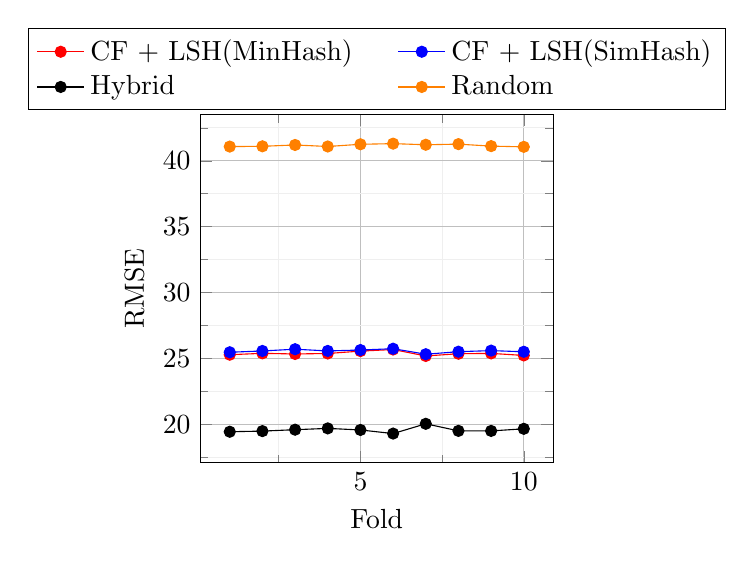
\begin{tikzpicture}
    \begin{axis}[
        xlabel=Fold,
        ylabel=RMSE,
        height=6cm,
        width = 0.5*\textwidth,
        grid = both,
        minor tick num = 1,
        ytick={5,10,15,20,25,30,35,40,45,50},
        major grid style = {lightgray},
        minor grid style = {lightgray!25},
        legend cell align = {left},
        legend columns=2,
        legend style={/tikz/every even column/.append style={column sep=0.5cm}, at={(0.5,1.25)},anchor=north}
    ]
    
    % Add values and attributes for the first plot
    \addplot[color=red,mark=*] coordinates {
        (1,25.296189214089544)
        (2,25.400462906839092)
        (3,25.352500267360195)
        (4,25.389339596960177)
        (5,25.570271635822632)
        (6,25.689527189672365)
        (7,25.201255678165264)
        (8,25.37051313093157)
        (9,25.39600667652665)
        (10,25.241320908436045)
    };
    
    % Add values and attributes for the second plot
    \addplot[color=blue,mark=*] coordinates {
        (1,25.482969708463497)
        (2,25.5812242180395)
        (3,25.7140533769646)
        (4,25.583410960871582)
        (5,25.65143951189667)
        (6,25.751353392266715)
        (7,25.334505039994312)
        (8,25.525532733650117)
        (9,25.60713940042656)
        (10,25.519782095279485)    
    };

    \addplot[color=black,mark=*] coordinates {
        (1,19.45607901371203)
        (2,19.503753114264153)
        (3,19.611318549782524)
        (4,19.709606837262)
        (5,19.590875207190635)
        (6,19.31785443100376)
        (7,20.0584529809771)
        (8,19.52192675987994)
        (9,19.51737504342661)
        (10,19.678156229689915)
    };

    \addplot[color=orange,mark=*] coordinates {
        (1,41.077744214275924)
        (2,41.098820791644044)
        (3,41.200106959030585)
        (4,41.08469399973035)
        (5,41.25194365186433)
        (6,41.30065080414065)
        (7,41.21625834754354)
        (8,41.26314247293824)
        (9,41.11250386933701)
        (10,41.0565444690093)
    };
    
    \legend{CF + LSH(MinHash), CF + LSH(SimHash), Hybrid, Random}
    \end{axis}
    \end{tikzpicture}
    
    \caption{\normalfont Root means square error measured on different folds of the synthetic dataset.}
    \label{fig:rmse_synthetic}
\end{figure}

